\documentclass[12pt,a4paper,openright,twoside]{book}
\usepackage[italian]{babel}
\usepackage[utf8]{inputenc}
\usepackage{fancyhdr}
\usepackage{indentfirst}
\usepackage{graphicx}
\usepackage{verbatim}

\pagestyle{fancy}

\oddsidemargin=30pt
\evensidemargin=20pt

% Sillabazione
\hyphenation{}

% Intestazione e piè di pagina
\pagestyle{fancy}\addtolength{\headwidth}{20pt}
\renewcommand{\chaptermark}[1]{\markboth{\thechapter.\ #1}{}}
\renewcommand{\sectionmark}[1]{\markright{\thesection \ #1}{}}
\rhead[\fancyplain{}{\bfseries\leftmark}]{\fancyplain{}{\bfseries\thepage}}
\cfoot{}

% Interlinea
\linespread{1.3}

\begin{document}

%
% Dedica
%
\begin{titlepage}
  % No numero di pagina
  \thispagestyle{empty}
  \topmargin=6.5cm
  \raggedleft
  \large
  \em A Chiara
  \newpage
  % Non numera l'ultima pagina a sinistra.
  \clearpage{\pagestyle{empty}\cleardoublepage}
\end{titlepage}


\pagenumbering{roman}

\chapter*{Introduzione}
\rhead[\fancyplain{}{\bfseries
INTRODUZIONE}]{\fancyplain{}{\bfseries\thepage}}
\lhead[\fancyplain{}{\bfseries\thepage}]{\fancyplain{}{\bfseries
INTRODUZIONE}}
\addcontentsline{toc}{chapter}{Introduzione}

``Comunicare, sempre'' è un imperativo sempre più assordante. In
quest'ottica, negli ultimi anni, si è diffusa rapidamente la
comunicazione vocale su sistemi VoIP, comunemente nota come
``telefonia via Internet''. Questa tecnologia permette conversazioni
audio/video tra due o più partecipanti senza limiti di distanza e di
tempo, al prezzo di una normale connessione Internet a banda larga e
di un computer. La voce viene digitalizzata dall'apparecchio del
mittente e incapsulata in pacchetti che vengono inviati al
destinatario via Internet. Poiché i dati percorrono reti progettate
per un utilizzo generico utilizzando protocolli \emph{best effort},
può accadere che in determinate circostanze la rete non sia in grado
di fornire un servizio adatto a una comunicazione VoIP.

Il traffico VoIP necessita infatti di infrastrutture di rete che
offrano garanzie di interattività e affidabilità. Con interattività si
intende un tempo sufficientemente ridotto tra il momento in cui un
frammento di voce viene pronunciato dal mittente e il momento in cui
lo stesso frammento viene udito dal destinatario; un ritardo troppo
marcato renderebbe difficile lo scambio di battute nel dialogo degli
interlocutori. Con affidabilità si intende invece la capacità della
rete di portare a destinazione la quasi totalità dei pacchetti
inviati; un'alta percentuale di perdite di pacchetti renderebbe la
comunicazione vocale incomprensibile.

Con la diffusione della banda larga (ADSL, fibra ottica), le reti
pubbliche e private riescono a garantire una qualità di servizio
adeguata al VoIP. Tuttavia, più recentemente, alle reti cablate a
banda larga si sono affiancate le reti senza fili, per esempio Mobile
WiMAX, WiFI (IEEE802.11/a/b/g/n), ZigBee, UMTS, GPRS, che stanno
diventando una realtà sempre più diffusa grazie alla loro semplicità
di installazione, praticità di utilizzo ed economicità dei
componenti. Lo scenario tipico consiste in una rete senza fili che,
attraverso uno o più \emph{access point}, offre accesso a una rete
broad band cablata per svariati dispositivi mobili; in questi casi il
traffico di rete deve attraversare almeno un segmento di rete wireless
prima di giungere alla rete via cavo.

Spesso le reti senza fili non garantiscono la qualità del servizio
richiesta dalle applicazioni VoIP. Il requisito di affidabilità viene
minato da interferenze, collisioni tra pacchetti e dall'indebolimento
del segnale radio che si verifica all'aumentare della distanza tra
dispositivo e access point. Il requisito di interattività viene invece
violato ogniqualvolta vi sia la necessità di ritrasmettere i pacchetti
che sono stati persi durante un'errore di trasmissione. Inoltre, i
dispositivi senza fili sono fisicamente in grado di muoversi
attraverso le aree di copertura di più reti, ma non possono cambiare
associazione di rete senza interrompere gli scambi di dati in corso,
problema che limita fortemente la mobilità e rende impossibile le
comunicazioni VoIP senza interruzioni.

È lecito immaginare che in un futuro prossimo la copertura delle reti
senza fili diventerà sempre più pervasiva, con città intere costellate
di punti di accesso a reti wireless di diversa tipologia. In questo
scenario sono necessari meccanismi e protocolli che permettano l'uso
di applicazioni VoIP in condizioni di estrema mobilità, garantendo le
proprietà di interattività e affidabilità necessarie.

In questo documento (TODO: tesi, lavoro, opera?) presenterò lo stato
dell'arte della qualità di servizio su sistemi VoWLAN, analizzando
alcune soluzioni presenti in letteratura, con particolare attenzione
alla soluzione proposta dall'attività di ricerca svolta all'interno
dell'Università di Bologna.

TODO: nel primo capitolo

TODO: nel secondo capitolo

TODO: etc.

% Non numera l'ultima pagina a sinistra.
\clearpage{\pagestyle{empty}\cleardoublepage}

% Indice
\tableofcontents
\rhead[\fancyplain{}{\bfseries\leftmark}]{\fancyplain{}{\bfseries\thepage}}
\lhead[\fancyplain{}{\bfseries\thepage}]{\fancyplain{}{\bfseries
INDICE}}
% Non numera l'ultima pagina a sinistra.
\clearpage{\pagestyle{empty}\cleardoublepage}

\chapter{Panoramica}
\lhead[\fancyplain{}{\bfseries\thepage}]{\fancyplain{}{\bfseries\rightmark}}
\pagenumbering{arabic}
L'obiettivo è di permettere a un MN di muoversi attraverso reti
wireless di natura eterogenea in maniera trasparente, ovvero senza
interrompere eventuali connessioni attive durante la transizione da
una rete all'altra. Perché questo sia possibile è necessario che ogni
MN sia a) univocamente identificato e b) universalmente raggiungibile
dagli altri nodi, in qualunque rete si trovi. Inoltre ogni MN dovrebbe
c) monitorare la qualità di ogni connessione wireless per poter
individuare la rete che offre le migliori garanzie di servizio e d)
eseguire un cambio di associazione trasparente per assicurare una
transizione senza interruzioni da una rete all'altra.

Le architetture proposte non hanno una collocazione ben precisa
all'interno dello stack di protocolli ISO/OSI.

Questo capitolo presenterà brevemente le soluzioni più importanti
presenti in letteratura, senza entrare nel merito dei singoli dettagli
tecnici, ma raggruppando e catalogando per tipo i vari approcci e
mostrando come ogni soluzione affronti ognuno dei quattro punti
chiave.

\section{Soluzioni \emph{single layer}}
Le architetture seguenti sono dette \emph{single layer} perché hanno
una collocazione ben precisa nello stack ISO/OSI e operano soltanto al
loro livello. L'analisi di queste soluzioni mostrerà i limiti
dell'approccio single layer, limiti che saranno superati dagli
approcci \emph{cross layer} descritti nella sezione successiva.

Queste architetture coprono i principali strati dello stack ISO/OSI:
Mobile IPv6 \cite{bib:mipv6} e la sua estensione Multiple Care-of
Addresses Registration \cite{bib:mcoa} agiscono a livello
\emph{network}, Host Identity Protocol \cite{bib:hip} definisce un
livello aggiuntivo tra \emph{network} e \emph{transport}, Datagram
Congestion Control Protocol \cite{bib:dccp} e Mobile Stream Control
Transport Protocol \cite{bib:m-sctp} lavorano a livello
\emph{transport}, infine Terminal Mobility Support Protocol
\cite{bib:tmsp} e MMUSE \cite{bib:mmuse} agiscono a livello
\emph{session}.

\subsection{Mobile IPv6 e Multiple Care-of Addresses Registration}
* Home Agent nella rete fa da LR\\
* Host parlano IPv6\\
* quindi infrastrutture di rete attuali non sono adatte\\
* no multi homing, perche' il protocollo non lo permette\\
* handover tribolato\\
MCoA\\
* estensione di MIPv6\\
* permette a MN di registrare più IP address con il suo Home Agent\\
* FlowMob permette di separare flussi di traffico tra le varie NIC\\
* stessi problemi di MIPv6: tutte le infrastrutture da cambiare.

\subsection{Host Identity Protocol}
* server tipo DNS opera fuori dalla rete di accesso\\
* mappa identificatori a posizioni\\
* il layer aggiuntivo deve essere installato sia nel MN che nel
  CN.\\
* Poco pratico! Non è detto che il CN si prenda la briga di installare\\
  il layer aggiuntivo.\\

\subsection{Datagram Congestion Control Protocol}
* ogni MN annuncia il cambiamento di rete all'altro nodo\\
* funziona solo se cambiano rete uno alla volta! Due MN che cambiano
  rete simultaneamente sono irragiungibili.\\
* richiedono modifica delle applicazioni.\\

\subsection{Mobile Stream Control Transport Protocol}
Idem a DCCP.

\subsection{Terminal Mobility Support Protocol}
* SIP user agent pubblico fuori dalle reti di accesso, mappa
  user@foo.com a posizione\\
* handover lento! ogni riconfigurazione interrompe la comunicazione
  finchè MN non ha finito di comunicare con l'user agent pubblico.

\subsection{MMUSE}
* server SIP, Session Border Controller (SBC) all'interno del
  sistema autonomo, che può essere composto da più reti wireless
  eterogenee.\\
* permette di attraversare i firewall e di spostarsi da una subnet
  all'altra all'interno dello stesso AS.\\
* MN non si può muovere tra reti di diversi AS.\\

\subsection{Considerazioni}
Tutte soluzioni tranne MMUSE hanno problemi con NAT e
firewall. Bisogna usare TURN e STUN. Tutte soluzioni senza
multi-homing, tranne MCoA.


\section{Soluzioni \emph{cross layer}}
Le architetture presenti sono dette \emph{cross layer} perché agiscono
a multipli livelli dello stack ISO/OSI, superando i limiti delle
architetture \emph{single layer} descritte in precedenza.

Il concetto di fondo di queste architetture è utilizzare le
informazioni disponibili al livello \emph{network} per poter prendere
decisioni efficaci di qualità di servizio ai livelli più alti.

Questa sezione confronterà le soluzioni ``Media Optimization Network
Architecture'' (MONA) e ``Always Best Packet Switching'' (ABPS).

Entrambe le architetture agiscono in uno scenario in cui ci sono
numerosi Mobile Node (MN), ognuno dotato di più interaccie di rete
(NIC), che operano in un ambiente dove sono disponibili più reti
wireless, eterogenee per tecnologia e dominio. Si immagina che i
movimenti degli utenti portino i vari MN ad attraversare le aree di
copertura delle reti wireless, per cui un MN connesso ad una
determinata rete A potrebbe spostarsi in un'area in cui giungono sia i
segnali della rete A che quelli di una seconda rete B, per poi
spostarsi ulteriormente nell'area di copertura della sola rete
B. Durante questi spostamenti l'utente deve essere in grado di
utilizzare applicazioni di rete real time, come Voice over IP e Video
on Demand, senza avere ripercussioni sulla qualità dell'esperienza. Il
traffico real time deve inoltre coesistere con il traffico non real
time delle applicazioni TCP/IP tradizionali, senza per questo venirne
penalizzato.

\subsection{Media Optimization Network Architecture}
%% Breve panoramica di MONA

MONA definisce uno strato aggiuntivo, posizionato tra gli strati
\emph{network} e \emph{transport} e denominato \emph{association
  layer}, che implementa l'Association Management Protocol (AMP);
detto protocollo risiete degli host e ne gestisce i singoli
collegamenti di rete, nascondendone la molteplicità allo strato
\emph{transport} superiore.

La molteplicità di collegamenti viene sfruttata per gestire il
problema dell'\emph{handover}, ovvero del passaggio dall'associazione
con una rete all'associazione con un'altra. In MONA ogni NIC tenta di
associarsi al proprio access point, e AMP decide se utilizzare una
sola NIC, quando il collegamento è soddisfacente, o se utilizzarne più
d'una contemporaneamente, quando il monitoraggio della NIC mostra
problemi di degrado delle prestazioni di rete.

MONA inoltre propone una modifica al comportamento degli access point
per supportare più efficientemente il traffico bidirezionale tipico
delle applicazioni VoIP e una aggiunta alle frame di \emph{probe} e
\emph{beacon} per permettere ai MN di selezionare l'access point con
migliore \emph{throughput}.

\subsection{Always Best Packet Switching}
%% Breve panoramica di ABPS

\subsection{Considerazioni}
Vantaggi delle due soluzioni rispetto a quelle single layer.

\clearpage{\pagestyle{empty}\cleardoublepage}


\chapter{Media Optimization Network Architecture}
Questo capitolo analizzerà nel dettaglio l'architettura MONA.

\clearpage{\pagestyle{empty}\cleardoublepage}


\chapter{Always Best Packet Switching}
Questo capitolo analizzerà nel dettaglio l'architettura ABPS.

\clearpage{\pagestyle{empty}\cleardoublepage}


\chapter{Considerazioni finali}
Riprende superiorità di cross layer su single layer e confronta punti
forti e deboli di MONA e ABPS.

Propone scenari di test?

\clearpage{\pagestyle{empty}\cleardoublepage}


%%%%%%%%%%%%%%%%%%%%%%%%%%%%%%%%%%%%%%%%%%%%%%%%%%%%%%%%%%%%%%%%%%%%%
%                   DA QUI IN POI E' ROBA VECCHIA                   %
%%%%%%%%%%%%%%%%%%%%%%%%%%%%%%%%%%%%%%%%%%%%%%%%%%%%%%%%%%%%%%%%%%%%%

\begin{comment}

% Capitoli
\chapter{Scenario}
\lhead[\fancyplain{}{\bfseries\thepage}]{\fancyplain{}{\bfseries\rightmark}}
\pagenumbering{arabic}

Lo scenario da considerare è illustrato in figura \ref{fig:scenario} e
originariamente presentato negli articoli \emph{Robust Wireless Medium
  Access for VoWLAN Applications: A Cross--Layer QoS Mechanism}
\cite{bib:rwma} e \emph{Always Best Packet Switching: the mobile VoIP
  case study} \cite{bib:abps}. Si assuma che esista una comunicazione
vocale tra due sistemi A e B, in figura rappresentati come ``Alice'' e
``Bob''. Il sistema A è un dispositivo mobile dotato di più di
un'interfaccia wireless, ognuna delle quali è associata con un diverso
access point. I vari access point possono appartenere a infrastrutture
di rete e domini differenti e quindi essere completamente indipendenti
l'uno dall'altro. Gli access point sono connessi a Internet attraverso
una connessione via cavo. Il sistema B è un dispositivo fisso,
connesso a Internet via cavo attraverso una comune allacciamento
Internet a banda larga, come ADSL o fibra ottica.
\begin{figure}[t]
\centering
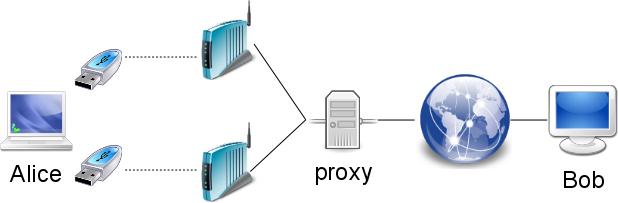
\includegraphics[width=\textwidth]{img/scenario}
\caption{Scenario}
\label{fig:scenario}
\end{figure}
La comunicazione VoIP tra i sistemi A e B si affida quindi a due tipi
di connessione: quella wireless, tra A e gli access point, e quella
via cavo tra gli access point e B.

\section{Vincoli qualitativi}
Come mostrato, il percorso dei dati da un sistema VoIP all'altro deve
attraversare segmenti camblati e altri senza fili; di questi gli
ultimi sono i più problematici, perché soffrono di tre gravi
inconvenienti: alta latenza, frequenti errori di trasmissione e
interruzione e ripristino della connessione nel cambiare access
point. Latenza ed errori frequenti possono degradare la qualità di una
comunicazione VoIP via wireless fino a renderla inintelleggibile,
mentre l'interruzione della connessione durante il passaggio da un
access point a un altro impedisce la mobilità del sistema obbligando
l'utente a restare nei pressi del ripetitore wireless in uso, pena la
disconnessione e l'interruzione della comunicazione.

Per garantire una buona qualità del servizio, il sistema RWMA deve
operare soddisfando vincoli di interattività, affidabilità e mobilità.

\subsection{Interattività}
L'interattività di una conversazione VoIP è influenzata dalla latenza
dei pacchetti che ne compongono il flusso di rete. La latenza di
trasmissione è definita come il tempo trascorso dall'istante del
campionamento della voce sul sistema di origine all'instante di
riproduzione audio della stessa voce sul sistema di destinazione. Le
raccomandazioni ITU--T \cite{bib:itu-t} indicano 150 ms come latenza
massima di una comunicazione VoIP soddisfacente; al di sopra di questa
soglia l'interattività della conversazione non è più accettabile.

\subsection{Affidabilità}
L'affidabilità di una conversazione VoIP dipende dalla capacità della
rete di portare a destinazione quanti più pacchetti possibili. Un
pacchetto è considerato perso quanto viene trasmesso dal sistema
origine e non viene ricevuto dal sistema destinazione. Per condurre
una conversazione comprensibile è necessario che la percentuale di
pacchetti persi resti al di sotto del 10\% \cite{bib:itu-t}. Poiché
per motivi di interattività le comunicazioni VoIP si svolgono su
protocollo UDP, la rete non offre nessun tipo di servizio di
trasmissione affidabile.

\subsection{Mobilità}
La mobilità dell'utente è fortemente limitata dallo scarso raggio
d'azione offerto dalle attuali apparecchiature WiFi. Le interfacce
WiFi sono in grado di interrompere l'associazione con l'access point
in uso per crearne una nuova con un secondo solo quando i suddetti
access point sono parte della stessa infrastruttura di rete. Questa
limitazione deriva direttamente dal funzionamento del protocollo IP:
cambiando rete di accesso l'interfaccia wireless riceve un nuovo
indirizzo IP e deve reinstaurare la connessione da zero. Ciò che si
vuole è invece un processo di disconnessione e riconnessione
trasparente all'applicazione, in modo che la chiamata VoIP non venga
interrotta, e rapido, in modo da non violare il requisito di
interattività precedentemente esposto.

\section{Il meccanismo RWMA}
Il meccanismo RWMA è costituito da più componenti, schematizzati in
figura \ref{fig:rwma}, che cooperano per risolvere i tre problemi di
interattività, affidabilità e mobilità. Questa sezione presenta
brevemente i componenti e illustra il loro ruolo nel progetto.
\begin{figure}[t]
\centering
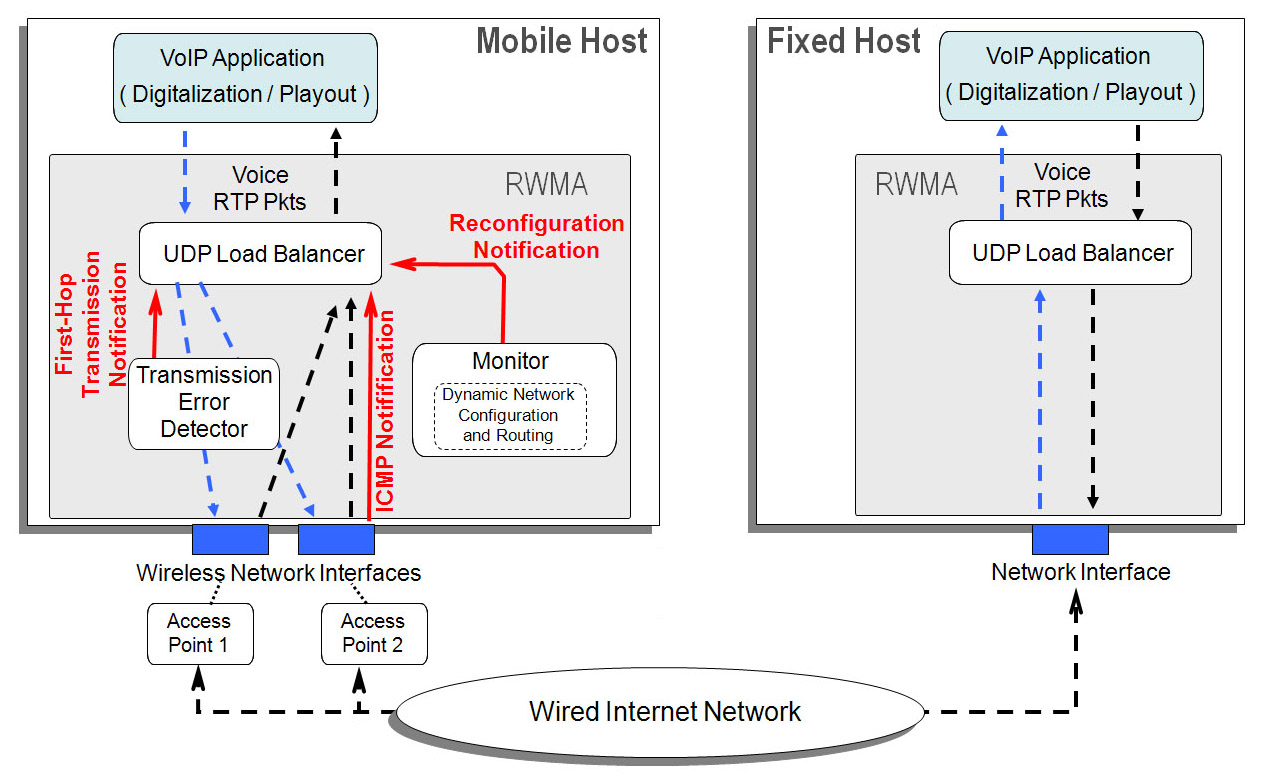
\includegraphics[width=\textwidth]{img/rwma}
\caption{Schema del meccanismo RWMA}
\label{fig:rwma}
\end{figure}

\subsection{Transmission Error Detection (TED)}
Questo componente software è integrato nel kernel del sistema
operativo del dispositivo mobile e ha il compito di tenere sotto
costante osservazione l'esito dell'invio dei pacchetti sulle
interfaccie wireless. Ogni volta che un'interfaccia WiFi invia un
\emph{frame} 802.11, questa deve attendere che l'access point risponda
con un frame di \emph{acknowledgment} che confermi l'avvenuta
ricezione. Nel caso in cui questo frame non venga ricevuto entro un
certo periodo di tempo, l'interfaccia ritenta la trasmissione fino a
un certo limite di volte, raggiunto il quale il frame viene
scartato. Se l'interfaccia riceve l'ACK, il firmware notifica il
kernel dell'avvenuta ricezione; al contrario, se il numero massimo di
tentativi viene raggiunto senza che l'interfaccia abbia ricevuto un
ACK, il firmware notifica il kernel del fallimento. Compito del TED è
rilevare queste notifiche positive e negative inviate dal firmware
dell'interfaccia e metterle a disposizione di applicazioni in
\emph{user space}.

\subsection{UDP Load Balancer (ULB)}
Questo componente software è un'applicazione in \emph{user space}
eseguita sul dispositivo mobile e ha il compito di rilevare le
notifiche di TED, e in base a queste decidere se rispedire i datagram
che non sono stati ricevuti dall'access point; inoltre deve valutare
di volta in volta quale sia l'interfaccia WiFi migliore da impiegare
per l'invio dei datagram.

\subsection{Interface Monitor (IM)}
Questo componente software lavora a stretto contatto con il gestore
delle interfacce wireless del sistema mobile e notifica ULB
dell'attivazione e della disattivazione di ogni interfaccia; dalle
notifiche di IM, ULB è quindi in grado di conoscere in ogni momento
quali interfacce wireless siano attive e associate a un'access point e
tra queste scegliere la migliore da usare per l'inoltro dei datagram.

\subsection{Proxy Server (PS)}
Questo componente software ha il compito di nascondere la mobilità del
sistema A, in modo che questo possa essere continuamente raggiungibile
dal sistema B. Il sistema B è in comunicazione con PS ed è
quest'ultimo a occuparsi di tenere traccia dei cambiamenti di
indirizzo IP che occorrono quando il sistema A cambia rete WiFi o
riattiva un'interfaccia di rete; come ULB, anche PS deve decidere a
quale interfaccia inoltrare i datagram ricevuti da B, ma a differenza
di ULB non si occupa di ritrasmettere eventuali pacchetti persi.

\chapter{Simulazione}
% Obiettivi a cui punto. Spiegazione soluzioni, algoritmi e scelte
% effettuate.
Tra i componenti del sistema RWMA descritti nel capitolo precedente,
UDP Load Balancer e Proxy Server ospitano il meccanismo su cui si basa
la qualità del servizio. Tutti gli altri meccanismi si occupano di
rilevare e trasmettere notifiche di errori o successi durante l'invio
di un datagram, quindi il comportamento è molto ben definito. ULB e PS
invece hanno il compito molto generico di dover scegliere
l'interfaccia \emph{migliore} per l'invio di ogni datagram. Gli
algoritmi di ULB e PS devono pertanto scegliere una definizione
operativa di ``migliore'' e applicarla alle interfacce WiFi in
uso.

In prima approssimazione un'interfaccia WiFi si può definire migliore
di un'altra quando offre maggiori probabilità di soddisfare i vincoli
di interattività e affidabilità descritti nel precedente capitolo; in
altre parole quando le stime di latenza e percentuale di pacchetti
persi per una data interfaccia sono le più basse tra le stime delle
altre interfacce attive.

Esistono vari modi per condurre queste stime, difficili da valutare
senza condurre test e misurazioni sul campo. La simulazione vuole
essere un banco di prova sperimentale virtuale, in cui condurre test
in maniera più comoda ed economica che nel mondo reale.

Scopo della simulazione è quindi confrontare diversi algoritmi di
stima della qualità delle interfacce WiFi per i componenti UDP Load
Balancer e Proxy Server.

Le sezioni successive mostreranno i problemi incontrati e le soluzioni
proposte.

\section{UDP Load Balancer}
Questa sezione illustra i problemi che devono essere affrontati dagli
algoritmi implementati dal componente ULB.

\subsection{Ritrasmissione in tempi brevi}
ULB deve attendere le notifiche del TED e ritrasmettere i datagram che
sono stati segnalati come persi, ma senza superare i 150 ms di
ritardo. Dopo tale periodo di tempo, un datagram voce viene
considerato \emph{stale} (scaduto) e quindi scartato. Inoltre la
ritrasmissione di un datagram causa l'attesa di tutti gli altri
datagram in coda; se ULB impiega troppi tentativi per ritrasmettere un
datagram, quelli successivi hanno meno tempo a disposizione per uscire
dal sistema prima di scadere. Il rischio è di far scadere una serie di
pacchetti solo per aver impiegato troppo tempo nella ritrasmissione di
uno. In particolare, ogni datagram contiene circa 40 ms di voce,
quindi ULB riceve i datagram da inoltrare a intervalli di circa 40 ms;
ogni datagram ha quindi 40 ms in cui può impegnare l'interfaccia
designata senza rubare tempo agli altri datagram in coda. Se ULB
dedica molto più di 40 ms all'invio di un datagram, rischia di
compromettere l'intera coda.

La soluzione proposta è di permettere una sola ritrasmissione per
datagram e di assegnare una valutazione negativa all'interfaccia che
ha ricevuto la notifica d'errore d'invio dal componente TED. In questo
modo la ritrasmissione di un pacchetto non blocca lo smaltimento degli
altri pacchetti in coda e la valutazione negativa all'interfaccia
problematica permette all'altra interfaccia designata per l'invio.

\subsection{Valutazione interfacce -- ULB}
ULB deve stimare la qualità di ogni interfaccia WiFi osservando le
notifiche ricevuto da TED.

TODO: algoritmo valutazione interfaccia, lo scrivo per ultimo a scanso
fix dell'ultimo momento.

\subsection{Rilevazione delle capacità del firmware}
I firmware delle schede di rete wireless sono in grado di notificare
sia l'avvenuta trasmissione di un datagram (ACK), sia la mancata
trasmissione (NACK). Normalmente le schede WiFi in commercio sono in
grado di notificare entrambi i casi, ma alcuni firmware sono in grado
di notificare solo ACK, oppure solo NACK. Mancando un meccanismo nel
kernel Linux per conoscere con certezza le capacità di ogni firmware,
ULB deve dedurrne il tipo dalle notifiche ricevute da TED. Conoscere a
priori il tipo di notifiche che possono giungere da un'interfaccia è
importante perché in caso di firmware che non possa segnalare i
fallimenti, ULB deve supplire a questa mancanza impostando un timeout
di ritrasmissione.

\subsubsection{Il problema del firmware silenzioso}
Il tipo di firmware si deduce dal tipo di notifiche ricevute dallo
stesso ed è quindi un meccanismo banale. Esistono però due casi in cui
il firmware può rimanere ``silenzioso'' e quindi impossibile da
rilevare: quando una connessione pessima, cioè che perde tutti i
pacchetti, viene gestita da un firmware ACK che notifica solo
successi, oppure quando una connessione ottima, ovvero che non perde
nessun pacchetto, viene gestita da un firmware NACK che notifica solo
fallimenti.

Non esiste un comportamento predefinito che soddisfi entrambe le
situazioni: la strategia del ritrasmettere ogni datagram che non
riceva notifiche entro un certo timeout funziona solo nella prima
situazione e risulta completamente inadeguato nella seconda.

\subsection{Valutazione interfacce -- PS}
Poiché il sistema mobile è dotato di più interfacce, PS si trova
nella necessità di scegliere a quale di queste debba inoltrare i dati
ricevuti dal sistema fisso.

La soluzione proposta consiste nel rispondere all'interfaccia che ha
spedito gli ultimi dati ricevuti; in altre parole inviare i dati
all'ultimo indirizzo IP da cui PS ha ricevuto traffico.

Può però accadere che il sistema mobile non invii alcun dato perché
l'utente si limita ad ascoltare; in questo caso il PS non ha
cognizione di quale sia l'interfaccia a cui inviare i dati.

TODO: soluzione PING, forse verrà già detta nella sezione ULB

\chapter{Simulatore}
Questo capitolo descrive brevemente l'implementazione del simulatore
progettato per la valutazione degli algoritmi ULB e PS.

Il simulatore è di tipo a eventi discreti ed è costituito da tre
strati.

Il primo strato è denominato \emph{de-sim} e costituisce un
\emph{framework} generico che definisce le classi di base da estendere
per modellare gli oggetti e i collegamenti, implementa la gestione di
eventi ed errori, l'instaurazione di collegamenti tra oggetti e
definisce primitive di input e output per lo scambio di oggetti tra
attori collegati.

Il secondo strato è denominato \emph{ulb-sim} e si basa su de-sim
estendendone le classi e specializzandone i metodi, per modellare una
versione semplificata del meccanismo RWMA.

Il terzo strato è denominato \emph{ulb-snr} e descrive lo scenario da
simulare instanziando le classi definite in ulb-sim e inizializzando
gli oggetti e gli eventi di partenza.

In altre parole, de-sim definisce come i meccanismi della simulazione,
ulb-sim gli oggetti partecipanti e infine ulb-snr dispone i
partecipanti nello scenario che si vuole raffigurare.

L'architettura a strati serve a mantenere indipendenza tra ciò che
definisce il ``cosa'' (ulb-sim) e ciò che definisce il ``come''
(ulb-snr): per esempio è possibile costruire nuovi scenari basati su
ulb-sim senza modificarne il codice.

Questra struttura è simile a quella del simulatore ns-2, in cui gli
oggetti della simulazione sono definiti da una gerarchia di classi in
C++, mentre gli scenari vengono definiti attraverso script Tcl
\cite{bib:ns-2}.

I tre strati sono scritti in Common Lisp \cite{bib:clhs}.

È importante notare che, a questo stadio di sviluppo, il simulatore
non punta al realismo fisico della simulazione. Per esempio, nelle
comunicazioni wireless non venendo presi in considerazione parametri
fisici come la qualità del segnale radio in relazione alla distanza
del client dall'access point. Tutti i dettagli di una connessione
wireless sono astratti dietro ai parametri di banda, latenza e
probabilità di errore; in particolare la rilevazione dell'ultimo
parametro sarà fondamentale per determinare la scelta dell'interfaccia
migliore. In quest'ottica, per simulare un calo di qualità del segnale
wireless dovuto all'aumentare della distanza tra client e access point
è sufficiente decidere quanto questo evento incida sulla probabilità
d'errore del collegamento e modificarla di conseguenza.

\chapter{Valutazioni}
TODO: Metriche con cui valuto il mio sistema. Deduzioni su misurazioni
effettuate. Perché ho misurato certe cose e non altre.

TODO: qui non ho la più pallida idea di cosa scrivere.

\chapter*{Conclusioni}
\rhead[\fancyplain{}{\bfseries
CONCLUSIONI}]{\fancyplain{}{\bfseries\thepage}}
\lhead[\fancyplain{}{\bfseries\thepage}]{\fancyplain{}{\bfseries
CONCLUSIONI}}
\addcontentsline{toc}{chapter}{Conclusioni}
TODO: che concludo?

\renewcommand{\chaptermark}[1]{\markright{\thechapter \ #1}{}}
\lhead[\fancyplain{}{\bfseries\thepage}]{\fancyplain{}{\bfseries\rightmark}}
\appendix
\chapter{Codice de-sim}
\rhead[\fancyplain{}{\bfseries Appendice \thechapter: Codice de-sim}]{\fancyplain{}{\bfseries\thepage}}
prova

\chapter{Codice ulb-sim}
\rhead[\fancyplain{}{\bfseries Appendice \thechapter: Codice ulb-sim}]{\fancyplain{}{\bfseries\thepage}}
prova

\end{comment}

\begin{thebibliography}{90}
\rhead[\fancyplain{}{\bfseries \leftmark}]{\fancyplain{}{\bfseries
\thepage}}
\addcontentsline{toc}{chapter}{Bibliografia}
\bibitem{bib:mipv6} RFC3775, ``Mobility Support in IPv6'',
  http://tools.ietf.org/html/rfc3775, giugno 2004
\bibitem{bib:mcoa} RFC5648, ``Multiple Care-of Addresses
  Registration'', http://tools.ietf.org/html/rfc5648, ottobre 2009
\bibitem{bib:hip} RFC5201 ``Host Identity Protocol'',
  http://tools.ietf.org/html/rfc5201, aprile 2008
\bibitem{bib:itu-t} ITU--T Recommendation G. 114, ``One--way
  Transmission'', maggio 2003
\bibitem{bib:abps} V. Ghini, G. Lodi, F. Panzieri, ``Always Best
  Packet Switching: the Mobile VoIP Case Study'', Achademy Plublisher,
  Journal of Communications, accepted for publication.
\bibitem{bib:ns-2} http://nsnam.isi.edu/nsnam/, ottobre 2009
\bibitem{bib:clhs}
  http://www.lispworks.com/documentation/HyperSpec/Front/,
  ottobre 2009
\end{thebibliography}
\end{document}
